\documentclass[a4paper]{article}
\usepackage{inputenc}
\usepackage[british,UKenglish]{babel}
\usepackage{amsmath}
%\usepackage{titlesec}
\usepackage{color}
\usepackage{graphicx}
\usepackage{fancyref}
\usepackage{hyperref}
\usepackage{float}
\usepackage{scrextend}
\usepackage{setspace}
\usepackage{xargs}
\usepackage{multicol}
\usepackage{nameref}

\usepackage{sectsty}
\usepackage{multicol}
\usepackage{multirow}
\usepackage[procnames]{listings}
\usepackage{appendix}

\newcommand\tab[1][1cm]{\hspace*{#1}}
\hypersetup{colorlinks=true, linkcolor=black}
\interfootnotelinepenalty=10000

\newcommand{\cleancode}[1]{\begin{addmargin}[3em]{3em}\texttt{\textcolor{cleanOrange}{#1}}\end{addmargin}}
\newcommand{\cleanstyle}[1]{\text{\textcolor{cleanOrange}{\texttt{#1}}}}


\usepackage[colorinlistoftodos,prependcaption,textsize=footnotesize]{todonotes}
\newcommandx{\commred}[2][1=]{\textcolor{Red}
{\todo[linecolor=red,backgroundcolor=red!25,bordercolor=red,#1]{#2}}}
\newcommandx{\commblue}[2][1=]{\textcolor{Blue}
{\todo[linecolor=blue,backgroundcolor=blue!25,bordercolor=blue,#1]{#2}}}
\newcommandx{\commgreen}[2][1=]{\textcolor{OliveGreen}{\todo[linecolor=OliveGreen,backgroundcolor=OliveGreen!25,bordercolor=OliveGreen,#1]{#2}}}
\newcommandx{\commpurp}[2][1=]{\textcolor{Plum}{\todo[linecolor=Plum,backgroundcolor=Plum!25,bordercolor=Plum,#1]{#2}}}

\def\code#1{{\tt #1}}

\def\note#1{\noindent{\bf [Note: #1]}}

\makeatletter
%% The "\@seccntformat" command is an auxiliary command
%% (see pp. 26f. of 'The LaTeX Companion,' 2nd. ed.)
\def\@seccntformat#1{\@ifundefined{#1@cntformat}%
   {\csname the#1\endcsname\quad}  % default
   {\csname #1@cntformat\endcsname}% enable individual control
}
\let\oldappendix\appendix %% save current definition of \appendix
\renewcommand\appendix{%
    \oldappendix
    \newcommand{\section@cntformat}{\appendixname~\thesection\quad}
}
\makeatother


% "define" Scala
\usepackage[T1]{fontenc}  
\usepackage[scaled=0.82]{beramono}  
\usepackage{microtype} 

\sbox0{\small\ttfamily A}
\edef\mybasewidth{\the\wd0 }

\lstdefinelanguage{scala}{
  morekeywords={abstract,case,catch,class,def,%
    do,else,extends,false,final,finally,%
    for,if,implicit,import,match,mixin,%
    new,null,object,override,package,%
    private,protected,requires,return,sealed,%
    super,this,throw,trait,true,try,%
    type,val,var,while,with,yield},
  sensitive=true,
  morecomment=[l]{//},
  morecomment=[n]{/*}{*/},
  morestring=[b]",
  morestring=[b]',
  morestring=[b]"""
}

\usepackage{color}
\definecolor{dkgreen}{rgb}{0,0.6,0}
\definecolor{gray}{rgb}{0.5,0.5,0.5}
\definecolor{mauve}{rgb}{0.58,0,0.82}

% Default settings for code listings
\lstset{frame=tb,
  language=scala,
  aboveskip=3mm,
  belowskip=3mm,
  showstringspaces=false,
  columns=fixed, % basewidth=\mybasewidth,
  basicstyle={\small\ttfamily},
  numbers=none,
  numberstyle=\footnotesize\color{gray},
  % identifierstyle=\color{red},
  keywordstyle=\color{blue},
  commentstyle=\color{dkgreen},
  stringstyle=\color{mauve},
  frame=single,
  breaklines=true,
  breakatwhitespace=true,
  procnamekeys={def, val, var, class, trait, object, extends},
  procnamestyle=\ttfamily\color{red},
  tabsize=2
}

\lstnewenvironment{scala}[1][]
{\lstset{language=scala,#1}}
{}
\lstnewenvironment{cpp}[1][]
{\lstset{language=C++,#1}}
{}
\lstnewenvironment{bash}[1][]
{\lstset{language=bash,#1}}
{}
\lstnewenvironment{verilog}[1][]
{\lstset{language=verilog,#1}}
{}


\usepackage{geometry}
\usepackage{graphicx}
\usepackage{appendix}
\usepackage{ctex}
\usepackage{lastpage}%获得总页数
\usepackage{tocloft}      %必须这么写,否则会报错
\usepackage{listings}
\usepackage{color}
\usepackage{multirow}
\usepackage{float}

\definecolor{mygreen}{rgb}{0,0.6,0}
\definecolor{mygray}{rgb}{0.5,0.5,0.5}
\definecolor{mymauve}{rgb}{0.58,0,0.82}

\lstset{ 
  backgroundcolor=\color{white},   % choose the background color; you must add \usepackage{color} or \usepackage{xcolor}; should come as last argument
  basicstyle=\footnotesize(or \small),        % the size of the fonts that are used for the code
  breakatwhitespace=false,         % sets if automatic breaks should only happen at whitespace
  breaklines=true,                 % sets automatic line breaking
  captionpos=b,                    % sets the caption-position to bottom
  caption = {}                     % set captions
  commentstyle=\color{mygreen},    % comment style
  deletekeywords={...},            % if you want to delete keywords from the given language
  escapeinside={\%*}{*)},          % if you want to add LaTeX within your code
  extendedchars=true,              % lets you use non-ASCII characters; for 8-bits encodings only, does not work with UTF-8
  firstnumber=1,                % start line enumeration with line 1000
  frame=single(or shadowbox),	   % adds a frame around the code
  keepspaces=true,                 % keeps spaces in text, useful for keeping indentation of code (possibly needs columns=flexible)
  keywordstyle=\color{blue},       % keyword style
  language=Octave,                 % the language of the code
  morekeywords={*,...},            % if you want to add more keywords to the set
  numbers=left,                    % where to put the line-numbers; possible values are (none, left, right)
  numbersep=5pt,                   % how far the line-numbers are from the code
  numberstyle=\tiny\color{mygray}, % the style that is used for the line-numbers
  rulecolor=\color{black},         % if not set, the frame-color may be changed on line-breaks within not-black text (e.g. comments (green here))
  showspaces=false,                % show spaces everywhere adding particular underscores; it overrides 'showstringspaces'
  showstringspaces=false,          % underline spaces within strings only
  showtabs=false,                  % show tabs within strings adding particular underscores
  stepnumber=1,                    % the step between two line-numbers. If it's 1, each line will be numbered
  stringstyle=\color{mymauve},     % string literal style
  tabsize=2,	                   % sets default tabsize to 2 spaces
  title=\lstname                   % show the filename of files included with \lstinputlisting; also try caption instead of title
  xleftmargin=4em,                 % set listing size through leftmargin
  xrightmargin=4em,                % set listing size through rightmargin
}  
\usepackage{listings}

%-------------------------页面边距--------------
\geometry{a4paper,left=2.3cm,right=2.3cm,top=2.7cm,bottom=2.7cm}
%-------------------------页眉页脚--------------
\usepackage{fancyhdr}
\pagestyle{fancy}
\lhead{\kaishu \leftmark}
% \chead{}
\rhead{\kaishu 计算机网络实验报告}%加粗\bfseries 
\lfoot{}
\cfoot{\thepage}
\rfoot{}
\renewcommand{\headrulewidth}{0.1pt}  
\renewcommand{\footrulewidth}{0pt}%去掉横线
\newcommand{\HRule}{\rule{\linewidth}{0.5mm}}%标题横线
\newcommand{\HRulegrossa}{\rule{\linewidth}{1.2mm}}
\setlength{\textfloatsep}{10mm}%设置图片的前后间距

\begin{document}
\renewcommand{\appendixname}{附录}
\renewcommand{\appendixpagename}{附录}
\renewcommand{\refname}{参考文献} 
\renewcommand{\figurename}{图}
\renewcommand{\tablename}{表}
\renewcommand{\today}{\number\year 年 \number\month 月 \number\day 日}
\newcommand\mydot[1]{\scalebox{#1}{.}}
\renewcommand\cftdot{\mydot{0.8}} % change the size of dots
\renewcommand\cftdotsep{3} % change the space between dots
%-------------------------封面----------------
\begin{titlepage}
    \begin{center}
    
\includegraphics[width=0.8\textwidth]{NKU.png}\\[1cm]
    \vspace{20mm}
		\textbf{\huge\textbf{\kaishu{计算机学院}}}\\[0.5cm]
		\textbf{\huge{\kaishu{计算机网络实验报告}}}\\[2.3cm]
		\textbf{\Huge\textbf{\kaishu{计算机网络大作业第四部分}}}
		\vspace{\fill}

    \centering
    \textsc{\LARGE \kaishu{姓名\ :\ 徐文斌}}\\[0.5cm]
    \textsc{\LARGE \kaishu{学号\ :\ 2010234}}\\[0.5cm]
    \textsc{\LARGE \kaishu{专业\ :\ 计算机科学与技术}}\\[0.5cm]
    \vfill
    {\Large \today}
    \end{center}
\end{titlepage}

\renewcommand {\thefigure}{\thesection{}.\arabic{figure}}%图片按章标号
\renewcommand{\contentsname}{目录} 
\cfoot{\thepage\ of \pageref{LastPage}}%当前页 of 总页数

% 生成目录
\clearpage
\tableofcontents
\newpage
%-------------------------内容----------------
\section{实验内容}

基于给定的实验测试环境,通过改变延迟时间和丢包率,完成下面3组性能对比实验:

\begin{enumerate}
    \item 停等机制与滑动窗口机制性能对比。
    \item 滑动窗口机制中不同窗口大小对性能的影响。
    \item 有拥塞控制和无拥塞控制的性能比较。
\end{enumerate}

\section{实验要求}

\begin{enumerate}
    \item 完成给定测试文件的传输,显示传输时间和平均吞吐率。
    \item 控制变量法。
    \item 性能测试指标包括吞吐率和时延,给出图形结果并进行分析。
\end{enumerate}

\section{实验结果}

\subsection{停等机制与滑动窗口机制性能对比}

这里我们固定最大报文端长度MSS为6666个字节。滑动窗口我们使用GBN算法,并固定窗口大小为10。
然后,我们测试程序的传输性能。首先,固定延时为0ms,分别取不同的丢包率。测试两种机制在
测试文件1.jpg上的吞吐率和传输时延,所得数据如表\ref{table:1}所示。

\begin{table}[!htbp]
\centering
\begin{tabular}{|cc|c|c|c|c|c|c|c|c|c|}
\hline
\multicolumn{2}{|c|}{丢包率} & 0 & 0.1 & 0.3 & 0.5 & 1 & 1.5 & 2 & 3 & 5 \\ \hline
\multicolumn{1}{|c|}{\multirow{2}{*}{时延}} & 停等机制 & 3.262 & 4.393 & 4.928 & 5.498 & 6.017 & 6.505 & 7.06 & 8.518 & 12.31 \\ \cline{2-11} 
\multicolumn{1}{|c|}{} & 滑动窗口 & 1.252 & 3.896 & 4.272 & 4.507 & 5.71 & 7.126 & 8.492 & 11.466 & 20.948 \\ \hline
\multicolumn{1}{|c|}{\multirow{2}{*}{吞吐率}} & 停等机制 & 569.39 & 422.80 & 376.89 & 337.82 & 308.68 & 285.53 & 263.08 & 218.05 & 150.88 \\ \cline{2-11} 
\multicolumn{1}{|c|}{} & 滑动窗口 & 1483.51 & 476.73 & 434.77 & 412.10 & 325.28 & 260.64 & 218.72 & 161.99 & 88.66 \\ \hline
\end{tabular}
\caption{停等机制与滑动窗口机制不同丢包率下文件传输时延(s)及吞吐率(KB/s)}
\label{table:1}
\end{table}

\begin{figure}[H]
  \centering
  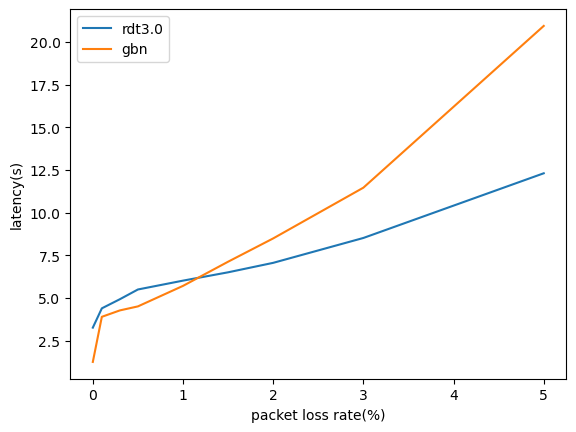
\includegraphics[width=0.7\textwidth]{f6.jpg}
  \caption{停等机制与滑动窗口机制不同丢包率下文件传输时延}
  \label{fig:7}
\end{figure}

\begin{figure}[H]
  \centering
  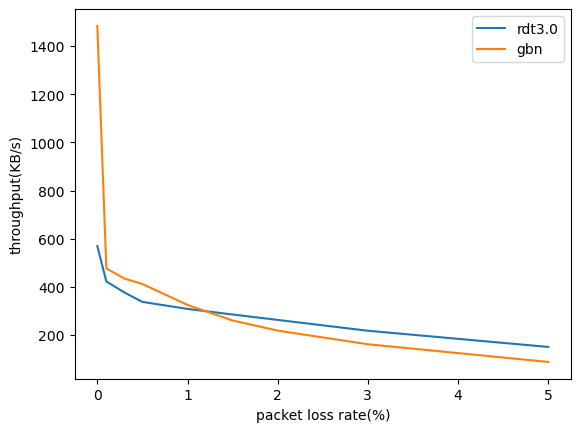
\includegraphics[width=0.7\textwidth]{f7.jpg}
  \caption{停等机制与滑动窗口机制不同丢包率下文件传输吞吐率}
  \label{fig:8}
\end{figure}

分析图\ref{fig:7}和图\ref{fig:8},我们可以发现,当丢包率较小时,滑动窗口机制性能优于
停等机制,而随着丢包率的增大,滑动窗口机制的时延开始大于停等机制。显然,当丢包率较小时,
与停等机制相比,滑动窗口一次能发送多个数据包,并且采用累积确认,可以有效利用网络带宽,
性能较好;而随着丢包率的增大,二者发生超时重传的次数也在逐渐增多,而GBN滑动窗口机制发生
超时时会重传当前窗口内的所有已发送但未确认的报文,开销较大,与之相比停等机制只会重传一个报文,重传开销
较小,因此,不难推断出,当丢包率较大时,GBN滑动窗口机制的超时重传开销过大,从而降低了其
文件传输性能。

下面,我们固定丢包率为0\%,分别取不同的延时。测试两种机制在文件1.jpg上的吞吐率和传输时延,
所得数据如表\ref{table:2}所示。不难发现,在测试的延时下,滑动窗口机制的性能均好于停等机制,
可见滑动窗口能更加充分地利用网络带宽,从而提升传输性能。

\begin{table}[!htbp]
\centering
\begin{tabular}{|cc|c|c|c|c|}
\hline
\multicolumn{2}{|c|}{延时(ms)} & 0 & 10 & 20 & 30 \\ \hline
\multicolumn{1}{|c|}{\multirow{2}{*}{时延(s)}} & 停等机制 & 3.262 & 9.572 & 14.215 & 17.625 \\ \cline{2-6} 
\multicolumn{1}{|c|}{} & 滑动窗口 & 1.252 & 8.858 & 13.259 & 15.21 \\ \hline
\multicolumn{1}{|c|}{\multirow{2}{*}{吞吐率(KB/s)}} & 停等机制 & 569.39086 & 194.04022 & 130.66148 & 105.38173 \\ \cline{2-6} 
\multicolumn{1}{|c|}{} & 滑动窗口 & 1483.5088 & 209.68085 & 140.08243 & 122.11394 \\ \hline
\end{tabular}
\caption{停等机制与滑动窗口机制不同延时下文件传输时延(s)及吞吐率(KB/s)}
\label{table:2}
\end{table}

\subsection{滑动窗口机制中不同窗口大小对性能的影响}

这里我们固定丢包率为0\%,延时为0ms,最大报文段长度为2300字节。设置GBN不同的窗口大小,测试程序传输文件1.jpg的时延和吞吐率。
测试结果如表\ref{table:3}及图\ref{fig:1}和图\ref{fig:2}所示。

\begin{table}[!htbp]
\centering
\begin{tabular}{|c|c|c|c|c|c|c|c|c|c|}
\hline
窗口大小 & 2 & 5 & 10 & 15 & 20 & 25 & 30 & 40 & 50 \\ \hline
时延(s) & 9.435 & 8.963 & 8.635 & 8.431 & 8.343 & 9.426 & 25.649 & 27.746 & 31.609 \\ \hline
吞吐率(KB/s) & 196.86 & 207.22 & 215.09 & 220.3 & 222.62 & 197.05 & 72.41 & 66.94 & 58.76 \\ \hline
\end{tabular}
\caption{滑动窗口机制中不同窗口大小文件传输时延及吞吐率}
\label{table:3}
\end{table}

\begin{figure}[H]
  \centering
  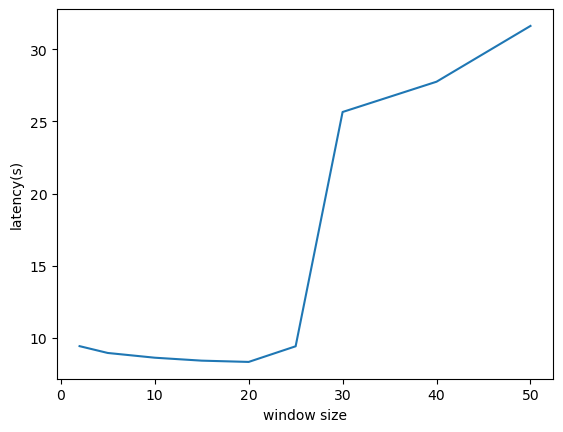
\includegraphics[width=0.7\textwidth]{f0.jpg}
  \caption{滑动窗口机制中不同窗口大小文件传输时延}
  \label{fig:1}
\end{figure}

\begin{figure}[H]
  \centering
  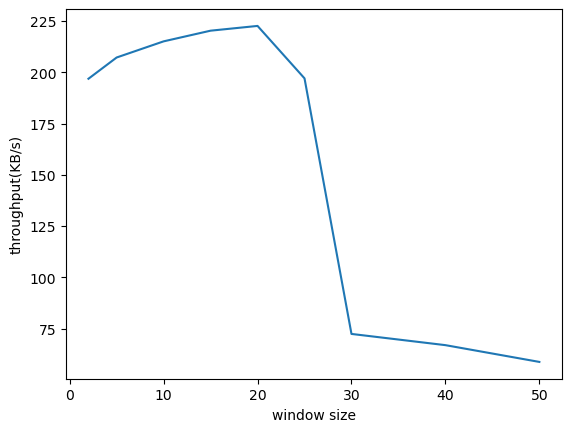
\includegraphics[width=0.7\textwidth]{f1.jpg}
  \caption{滑动窗口机制中不同窗口大小文件传输吞吐率}
  \label{fig:2}
\end{figure}

根据图表可以看出,随着窗口逐渐增大,发送端可以发送多个包,发包效率提升,吞吐率也增加。
当窗口数达到20左右,吞吐率达到顶峰,之后继续增大窗口,容易造成网络堵塞,由于接收端的
缓冲区大小有限,一次性发送太多数据包会导致产生丢包现象,从而增大文件传输时延,吞吐率
开始下降。可以看到,窗口大小在25-30左右,吞吐率发生了大幅度的下降。

\subsection{有拥塞控制和无拥塞控制的性能比较}

使用reno拥塞控制算法。这里我们固定窗口大小为15,对文件1.jpg进行传输测试。
分别改变丢包率和延时,比较无拥塞控制和有拥塞控制的算法的性能差异。结果如下所示。

\subsubsection{不同丢包率,无延时}

\begin{table}[!htbp]
\centering
\begin{tabular}{|cc|c|c|c|c|}
\hline
\multicolumn{2}{|c|}{丢包率} & 0\% & 1\% & 3\% & 5\% \\ \hline
\multicolumn{1}{|c|}{\multirow{2}{*}{时延(s)}} & 无拥塞控制 & 5.76 & 15.625 & 36.688 & 110.214 \\ \cline{2-6} 
\multicolumn{1}{|c|}{} & 有拥塞控制 & 4.831 & 13.149 & 27.028 & 40.629 \\ \hline
\multicolumn{1}{|c|}{\multirow{2}{*}{吞吐率(KB/s)}} & 无拥塞控制 & 322.457 & 118.871 & 50.626 & 16.852 \\ \cline{2-6} 
\multicolumn{1}{|c|}{} & 有拥塞控制 & 384.545 & 141.254 & 68.72 & 45.715 \\ \hline
\end{tabular}
\caption{有拥塞控制和无拥塞控制不同丢包率下文件传输时延及吞吐率}
\label{table:4}
\end{table}

\begin{figure}[H]
  \centering
  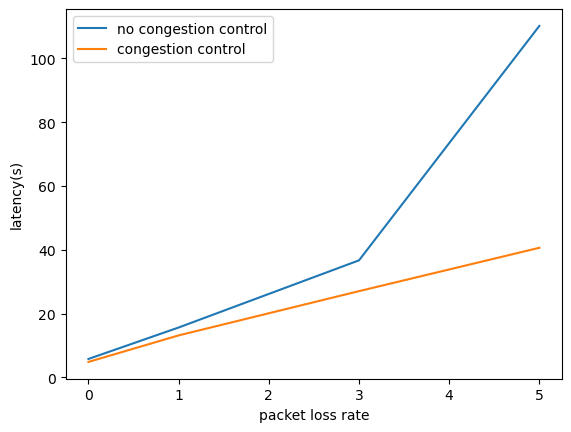
\includegraphics[width=0.7\textwidth]{f2.jpg}
  \caption{有拥塞控制和无拥塞控制不同丢包率下文件传输时延}
  \label{fig:3}
\end{figure}

\begin{figure}[H]
  \centering
  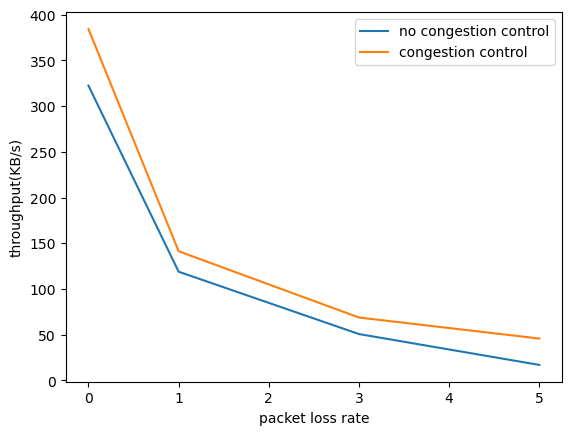
\includegraphics[width=0.7\textwidth]{f3.jpg}
  \caption{有拥塞控制和无拥塞控制不同丢包率下文件传输吞吐率}
  \label{fig:4}
\end{figure}

从图\ref{fig:3}中我们可以看到,随着丢包率的增大,有拥塞控制和无拥塞控制的滑动窗口算法
的文件传输时延都在增加,但我们可以明显的看到,有拥塞控制的滑动窗口算法的文件传输时延增加
速率更慢。显然,这是由于拥塞控制算法在产生丢包时及时限制了窗口的大小,从而避免了更进一步的网络拥塞
的产生。

进一步思考,当出现丢包的情况,无拥塞控制的滑动窗口只能等到触发超时才会重传报文,丢包率
越高,吞吐率越低;而拥塞窗口机制在收到三次重复ACK会触发快速重传,或者超时的情况下重传数据包,
因此拥塞控制机制在丢包的情况可以有更好的性能。综上,如果存在丢包的情况,有拥塞控制机制要明显
优于无拥塞控制机制的滑动窗口性能。

\subsubsection{不同延时,丢包率1\%}

\begin{table}[!htbp]
\centering
\begin{tabular}{|cc|c|c|c|c|}
\hline
\multicolumn{2}{|c|}{延时(ms)} & 0 & 1 & 3 & 5 \\ \hline
\multicolumn{1}{|c|}{\multirow{2}{*}{时延(s)}} & 无拥塞控制 & 17.617 & 40.205 & 42.041 & 61.412 \\ \cline{2-6} 
\multicolumn{1}{|c|}{} & 有拥塞控制 & 13.149 & 35.689 & 35.787 & 36.491 \\ \hline
\multicolumn{1}{|c|}{\multirow{2}{*}{吞吐率(KB/s)}} & 无拥塞控制 & 105.42959 & 46.197065 & 44.179563 & 30.244138 \\ \cline{2-6} 
\multicolumn{1}{|c|}{} & 有拥塞控制 & 141.25432 & 52.0427303 & 51.900215 & 50.898934 \\ \hline
\end{tabular}
\caption{有拥塞控制和无拥塞控制不同延时下文件传输时延及吞吐率}
\label{table:5}
\end{table}

\begin{figure}[H]
  \centering
  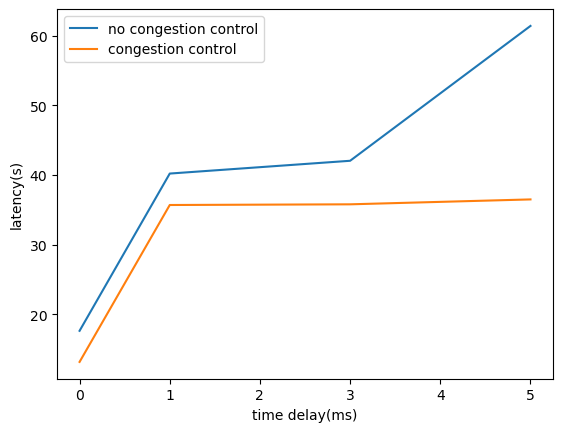
\includegraphics[width=0.7\textwidth]{f4.jpg}
  \caption{有拥塞控制和无拥塞控制不同延时下文件传输时延}
  \label{fig:5}
\end{figure}

\begin{figure}[H]
  \centering
  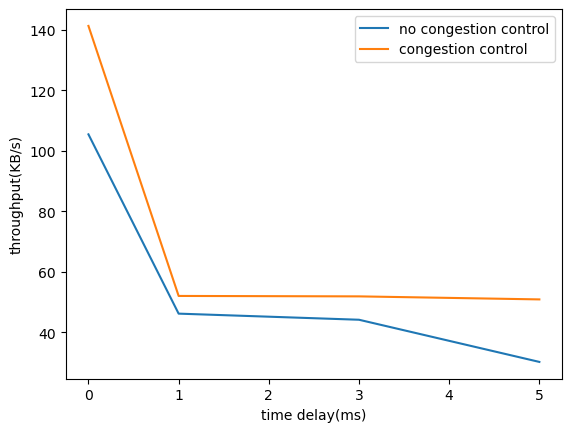
\includegraphics[width=0.7\textwidth]{f5.jpg}
  \caption{有拥塞控制和无拥塞控制不同延时下文件传输吞吐率}
  \label{fig:6}
\end{figure}

分析图\ref{fig:5}和图\ref{fig:6},对比延时为0ms和延时为1ms时文件的传输效率,可以发现延时对于文件传输的影响还是比较大的。
随着延时增大,文件传输效率降低。当出现延时的情况,无拥塞控制机制的滑动窗口的窗口大小不变,每次都发相同数量的包,在延时的
情况下,需要等待十分长的时间,容易造成超时发生;而拥塞控制机制在超时的情况下会调整窗口大小,将窗口重新设置为1,从而限制了
发送端的发送。因此延时变长对拥塞窗口机制的吞吐率影响小于对无拥塞控制机制的滑动窗口的影响。所以如果存在延时的情况,拥塞控制
机制要优于无拥塞控制的滑动窗口机制。

\end{document}